Events with an energetic jet $\pt$ and large $\met$ in the final state, constitute a
clean signature for new physics searches at hadron colliders. Signals that can
be studied with this experimental signature include the production of WIMPS,
the ADD model for large extra dimensions and SUSY.

\mbox{}

\noindent \textbf{Fix this part}

If the mass difference between the sparticles is small, the sensitivity to new
physics signal of many standard SUSY searches is reduced due to the low amount
of missing energy and the corresponding low transverse momentum of the
associated jets. (why is that so? Try to think and find out) If the event has an
ISR, the amount of missing energy and the corresponding transverse momentum jets
will be large leading thus to a clean signature for the monojet

\mbox{}

It is possible to estimate, from eq.~\eqref{eq:delta_mh}, the scale at which new
physics is expected. Using m$_H$ = 125~GeV~\cite{PDG}, we get that
$\Lambda \approx 1$~TeV; thus, if the naturalness criterion holds, we expect the
two main experiments at LHC, ATLAS and CMS, to find signal for new physics at
the TeV scale.

\begin{figure}[!h]
  \centering
  \begin{subfigure}[t]{.48\linewidth}
    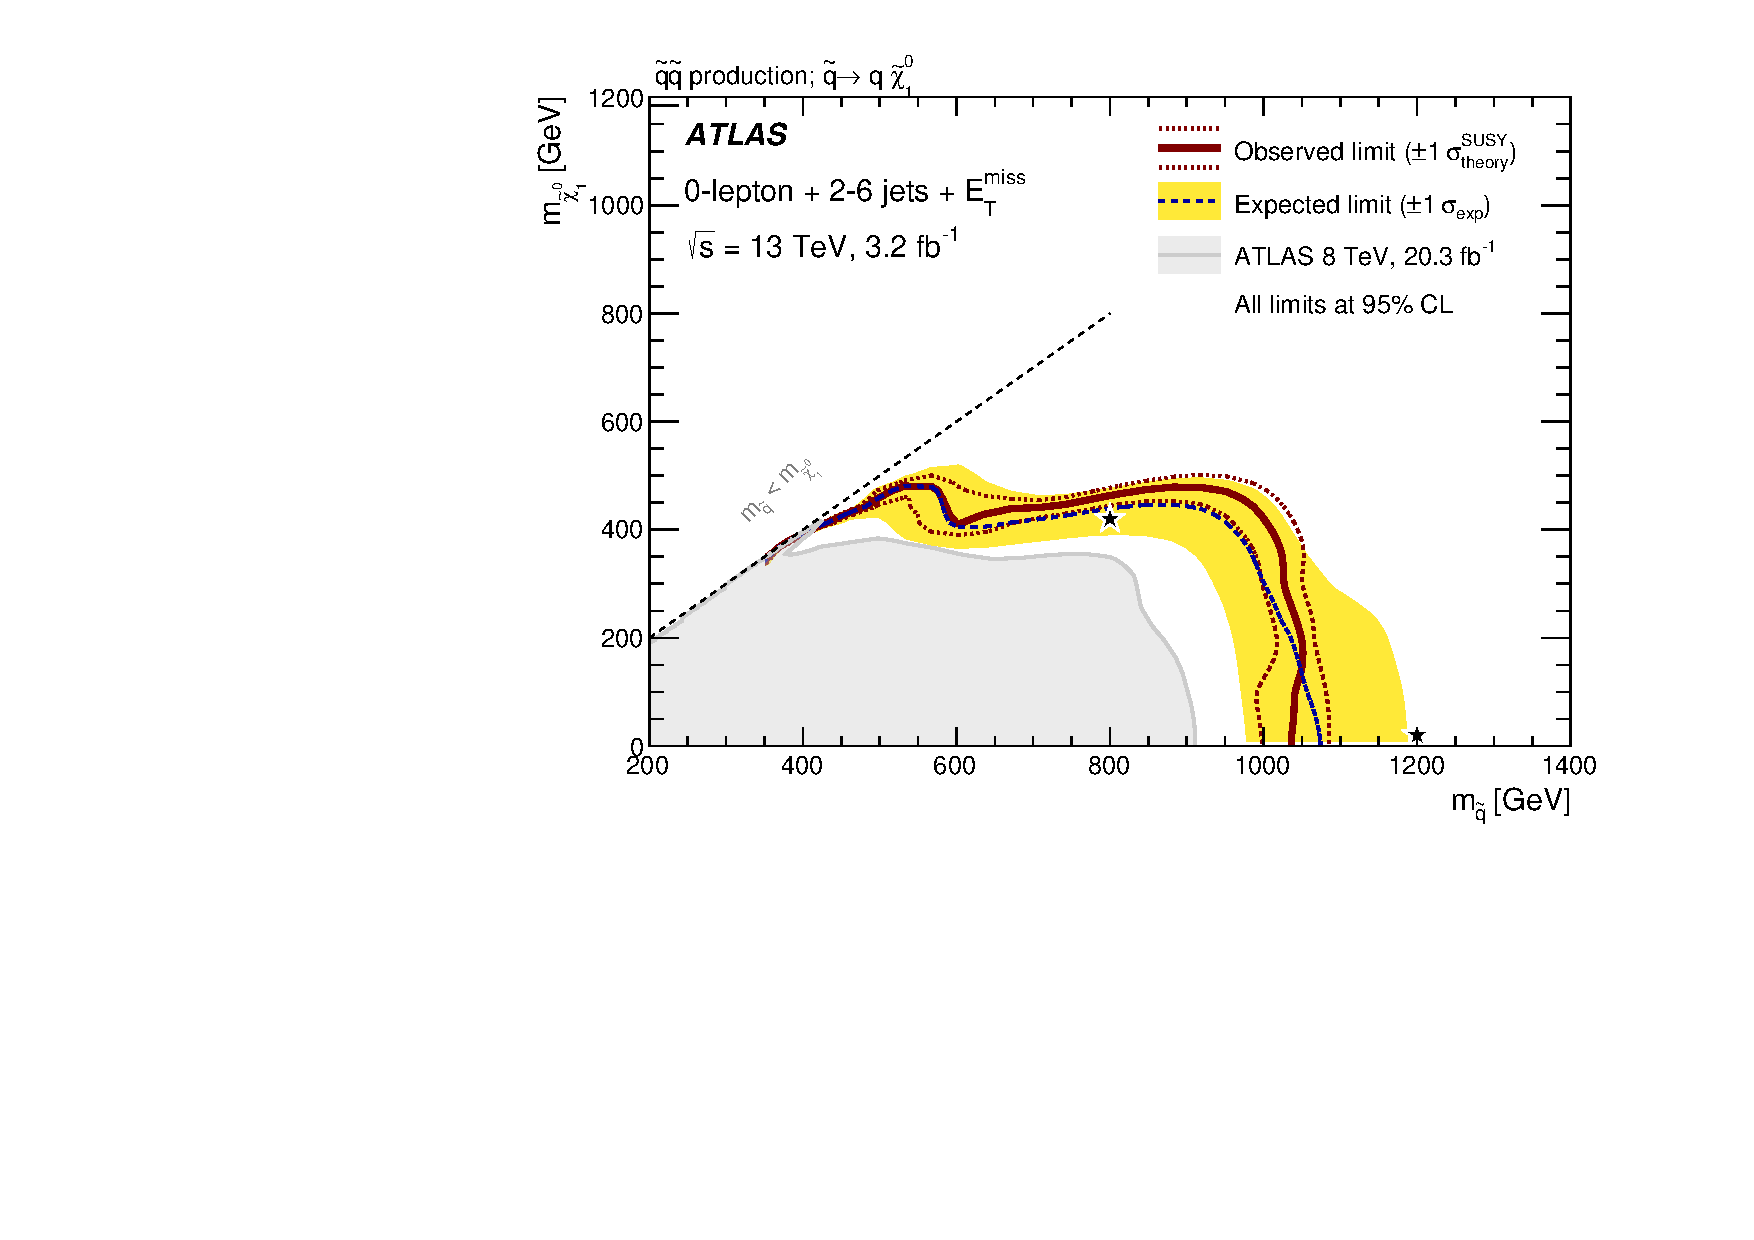
\includegraphics[width=\linewidth]{susy}
    \caption{}
    \label{fig:susy}
  \end{subfigure}
  \begin{subfigure}[t]{.48\linewidth}
    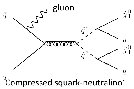
\includegraphics[width=\linewidth]{compressed}
    \caption{}
    \label{fig:compressed}
  \end{subfigure}
  \caption{}
  \label{fig:motivation}
\end{figure}
%%% Local Variables:
%%% mode: latex
%%% TeX-master: "../search_for_DM_LED_with_ATLAS"
%%% End:
